%
% aufgabe.tex -- Variationsaufgabe
%
% (c) 2021 Prof Dr Andreas Müller, OST Ostschweizer Fachhochschule
%
\bgroup
\begin{frame}[t]
\setlength{\abovedisplayskip}{5pt}
\setlength{\belowdisplayskip}{5pt}
\frametitle{Variationsaufgabe}
\vspace{-20pt}
\begin{columns}[t,onlytextwidth]
\only<1-11>{%
\begin{column}{0.48\textwidth}
\begin{block}{Brachistochrone\strut}
Man finde die Kurve $(x(\varphi),y(\varphi))$ derart, dass die Zeit
\[
t
=
\int
\frac{\sqrt{1 + y'(x)^2}}{v(y(x))}
\,dx
\]
minimal wird.
\end{block}
\uncover<2->{%
\begin{block}{Integrand enthält}
\begin{itemize}
\item<3-> die unbekannte Funktion $y(x)$
\item<4-> die Ableitung $y'(x)$
\item<5-> $v$ könnte auch noch von $x$ abhängen
\end{itemize}
\end{block}}
\end{column}}%
\begin{column}{0.48\textwidth}
\uncover<6->{%
\begin{block}{Allgemeines Problem\strut}
Gegeben:
\begin{itemize}
\item<7-> Funktion $L(x,y,y')$
\item<8-> Punkte $(x_1,y_1)$ und $(x_2,y_2)$
\end{itemize}
\uncover<9->{%
Gesucht: Funktion $y(x)$ derart, dass
\begin{itemize}
\item<10->
$y(x_k)=y_k$\quad für $k=1,2$
\item<11->
Das Integral
\[
I(y)
=
\int_{x_1}^{x_2}
L(x,y(x),y'(x))\,dx
\]
ist minimal}
\end{itemize}
\end{block}}
\only<24-26>{%
\begin{block}{Lösung}
\only<24>{Bernoulli's Trick funktioniert nicht}
\only<25->{Ableiten, Nullsetzen?}
\only<26>{Wonach?!}
\end{block}}
\end{column}
\only<12->{%
\begin{column}{0.48\textwidth}
\begin{center}
\def\xone{1}
\def\xtwo{5}
\def\yone{2}
\def\ytwo{5}
\pgfmathparse{(\ytwo-\yone)/(\xtwo-\xone)}
\xdef\m{\pgfmathresult}
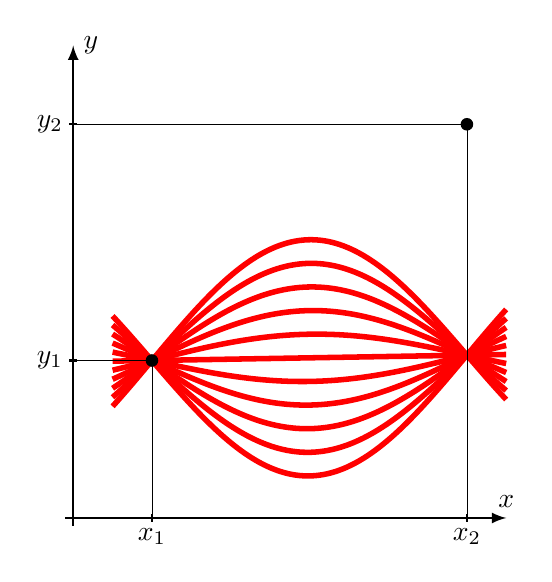
\begin{tikzpicture}[>=latex,thick]
% plot
\foreach \n in {13,...,23}{
\uncover<\n->{
	\pgfmathparse{0.3*(\n-18)}
	\xdef\t{\pgfmathresult}
	\draw[color=red,line width=2pt]
		plot[domain=0.5:5.5,samples=100]
			({\x},{\m*(\x-\xone)+\yone+\t*sin(180*(\x-\xone)/(\xtwo-\xone))});
}
}
% x1
\draw[line width=0.3pt] (\xone,\yone) -- (\xone,0);
\fill (\xone,\yone) circle[radius=0.08];
\draw (\xone,-0.05) -- (\xone,0.05);
\node at (\xone,0) [below] {$x_1$};
\draw[line width=0.3pt] (0,\yone) -- (\xone,\yone);
\draw (-0.05,\yone) -- (0.05,\yone);
\node at (0,\yone) [left] {$y_1$};
% x2
\draw[line width=0.3pt] (\xtwo,\ytwo) -- (\xtwo,0);
\fill (\xtwo,\ytwo) circle[radius=0.08];
\draw (\xtwo,-0.05) -- (\xtwo,0.05);
\node at (\xtwo,0) [below] {$x_2$};
\draw[line width=0.3pt] (0,\ytwo) -- (\xtwo,\ytwo);
\draw (-0.05,\ytwo) -- (0.05,\ytwo);
\node at (0,\ytwo) [left] {$y_2$};
% coordinate system
\draw[->] (-0.1,0) -- (5.5,0) coordinate[label={$x$}];
\draw[->] (0,-0.1) -- (0,6) coordinate[label={right:$y$}];
\end{tikzpicture}
\end{center}
\end{column}}%
\end{columns}
\end{frame}
\egroup
